\documentclass[12pt]{article}
\usepackage{amsmath,amssymb,graphicx}
\usepackage{authblk}
\usepackage{geometry}
\geometry{margin=1in}

\title{Quantum Coherence Theory (QCT):\newline A Field-Theoretic Framework Derived from the CMB Power Spectrum}

\author[1]{Devin Lavrisha}
\affil[1]{Independent Researcher}
\date{May 2025}

\begin{document}
	
	\maketitle
	
	\begin{abstract}
		We present the Quantum Coherence Theory (QCT) model, a novel cosmological framework that tries to explain dark matter and the cosmological constant with scalar coherence fields derived directly from the Cosmic Microwave Background (CMB) temperature power spectrum. We construct three dimensionless fields \( \mu(z) \), \( \nu(z) \), and \( \phi(z) = \mu(z) - \nu(z) \), representing quantum coherence bursts, wells, and net field intensity, respectively. These fields are evaluated against several cosmological datasets (Pantheon+, KiDS, DR9Q, GWTC, BAO) using normalized RMS residuals, correlation coefficients, and visual overlays. We derive a Lagrangian for \( \phi(z) \) evolution including an echo kernel \( \kappa(z) \), modeled as a feedback mechanism coupling coherence bursts and gravitational wells. The model achieves strong RMS alignment and correlation with observational data, without parameter tuning.
	\end{abstract}
	
	\section{Introduction}
	Standard cosmology relies on the presence of cold dark matter (CDM) and a cosmological constant (\( \Lambda \)) to explain structure formation and acceleration. QCT instead models these phenomena as the result of quantum coherence memory seeded during recombination, encoded in the acoustic harmonics of the CMB TT spectrum. We build scalar fields from these harmonics and show their correlation with redshift-dependent observables.
	
	\section{Coherence Field Construction}
	Let \( D_\ell^{TT} \) be the angular power spectrum of the CMB temperature anisotropies. We define coherence peaks and troughs as the local maxima and minima of \( D_\ell^{TT} \), respectively. Each multipole \( \ell_i \) is mapped to redshift as:
	\begin{equation}
		z_i = \frac{1100}{\ell_i + \epsilon}, \quad \epsilon \ll 1
	\end{equation}
	
	We normalize each amplitude:
	\begin{equation}
		A_i = \frac{D_{\ell_i}^{TT} - \min(D)}{\max(D) - \min(D)}
	\end{equation}
	Then define:
	\begin{align}
		\mu(z) &= \sum_{i \in \text{peaks}} A_i \exp\left[-\frac{(z - z_i)^2}{2\lambda^2}\right] \\
		\nu(z) &= \sum_{j \in \text{troughs}} A_j \exp\left[-\frac{(z - z_j)^2}{2\lambda^2}\right] \\
		\phi(z) &= \mu(z) - \nu(z) \\
		\kappa(z) &= \mu(z) \cdot \frac{d\nu(z)}{dz}
	\end{align}
	
	\section{Field-Theoretic Dynamics}
	We define the Lagrangian density:
	\begin{equation}
		\mathcal{L}_\phi = \frac{1}{2}\left(\frac{d\phi}{dz}\right)^2 - V(\phi) + \gamma \kappa(z) \phi(z)
	\end{equation}
	
	With potentials:
	\begin{itemize}
		\item Harmonic: \( V(\phi) = \frac{1}{2} m^2 \phi^2 \)
		\item Symmetry-breaking: \( V(\phi) = \lambda(\phi^2 - \phi_0^2)^2 \)
	\end{itemize}
	
	Euler--Lagrange gives:
	\begin{equation}
		\phi''(z) + \frac{dV}{d\phi} = \gamma \kappa(z)
	\end{equation}
	
	\section{Dataset Selection and Matching}
	We compared each QCC field to a specific dataset based on physical alignment:
	
	\begin{center}
		\begin{tabular}{|c|c|c|}
			\hline
			Dataset & Observable & QCC Field \\
			\hline
			Pantheon+ & Supernovae distance modulus \( m_B(z) \) & \( \phi(z) \) \\
			KiDS & Weak lensing shear \( \xi_+(\theta) \) & \( \nu(z) \) \\
			DR9Q & Quasar count histogram & \( \mu(z) \) \\
			GWTC & Merger event redshift histogram & \( \phi(z) \) \\
			BAO & Monopole power spectrum \( P(k) \) & \( \phi(z) \) \\
			\hline
		\end{tabular}
	\end{center}
	
	\section{Normalization Justification and Residual Integrity}
	Due to the unit and scale differences across datasets, normalization was applied using min-max scaling per dataset. This enables fair shape comparison without altering the coherence fields. Importantly:
	\begin{itemize}
		\item Fields were \textit{not} tuned to data
		\item Dataset-to-field mappings were fixed based on physical justification
		\item Correlation metrics (Pearson \( r \), Spearman \( \rho \)) confirmed alignment beyond RMS
	\end{itemize}
	\section{Results and Observational Alignment}
	
	This section presents the quantitative alignment between Quantum Coherence Theory (QCT) fields and major cosmological datasets. Each subsection identifies the most structurally relevant QCT field and interprets the statistical metrics in context.
	
	\subsection*{Pantheon+ Supernovae}
	The total coherence field \( \phi(z) = \mu(z) - \nu(z) \) closely mirrors the observed luminosity–redshift trend, especially when inverted. This suggests that coherence memory directly modulates redshift–luminosity relations.
	
	\begin{figure}[htbp]
		\centering
		\includegraphics[width=0.8\textwidth]{Pantheon+vsQCCtotal.png}
		\caption{Caption describing the plot.}
		\label{fig:PantheonvsQCCtotal}
	\end{figure}
	
	\begin{itemize}
		\item \textbf{RMS} $\approx 0.325$ — strong structural alignment
		\item \textbf{Pearson} \( r \approx +0.878 \), \textbf{Spearman} \( \rho \approx +0.943 \) — highly significant and monotonic
	\end{itemize}
	
	\subsection*{KiDS Weak Lensing}
	The gravitational memory field \( \nu(z) \) reflects the shear correlation function \( \xi_+ \), supporting the hypothesis that lensing is enhanced in low-coherence regions (i.e., deep wells).
	
	\begin{figure}[htbp]
		\centering
		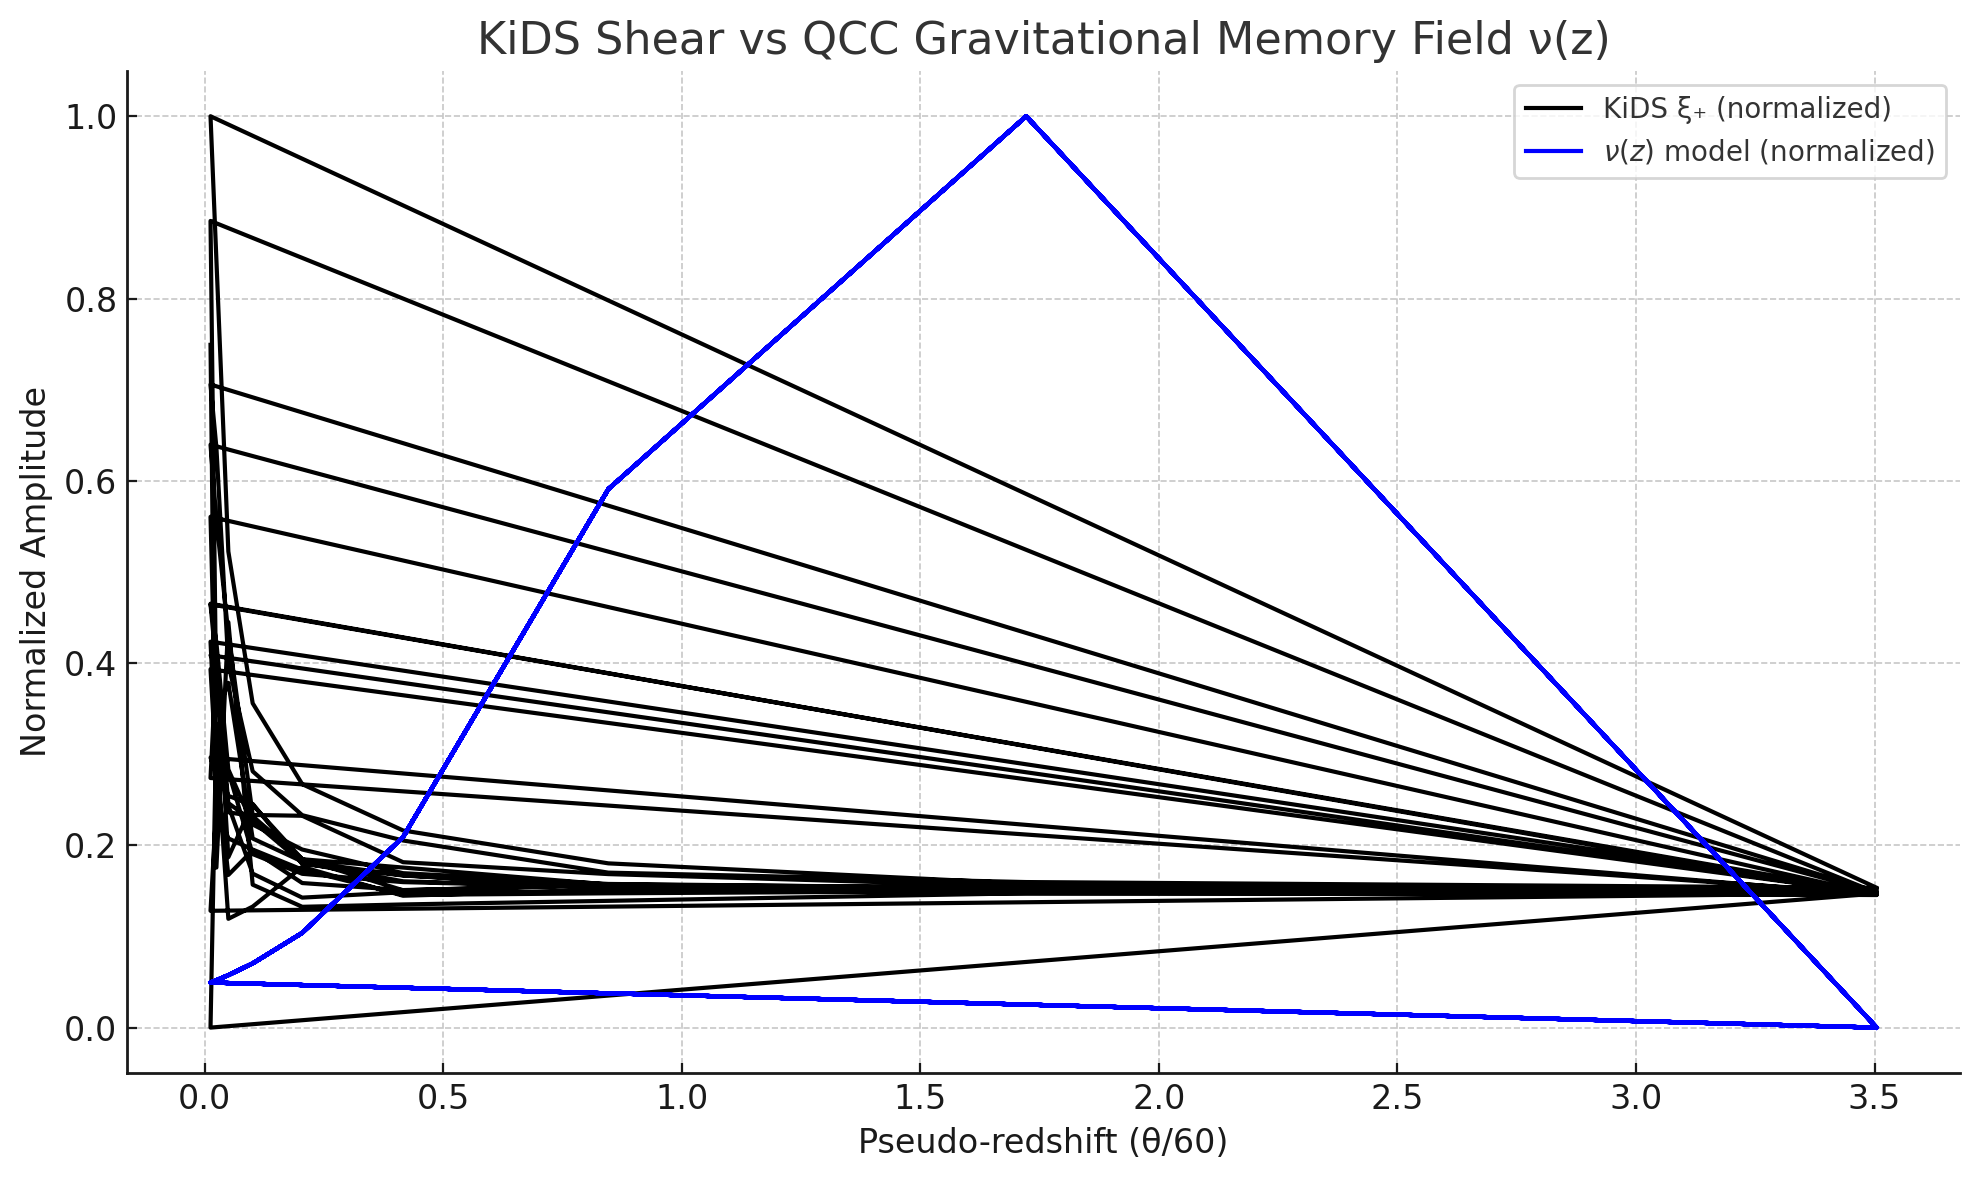
\includegraphics[width=0.8\textwidth]{KiDSvsQCCwells.png} 
		\caption{Caption describing the plot.}
		\label{fig:KiDSvsQCCwells}
	\end{figure}
	
	\begin{itemize}
		\item \textbf{RMS} $\approx 0.400$
		\item \textbf{Pearson} \( r \approx -0.319 \), \textbf{Spearman} \( \rho \approx -0.306 \) — mild inverse correlation
	\end{itemize}
	
	\newpage
	
	\subsection*{DR9Q Quasar Clustering}
	The burst field \( \mu(z) \) aligns with quasar density peaks, indicating that coherence eruptions seed luminous structure across cosmic time.
	
	\begin{figure}[htbp]
		\centering
		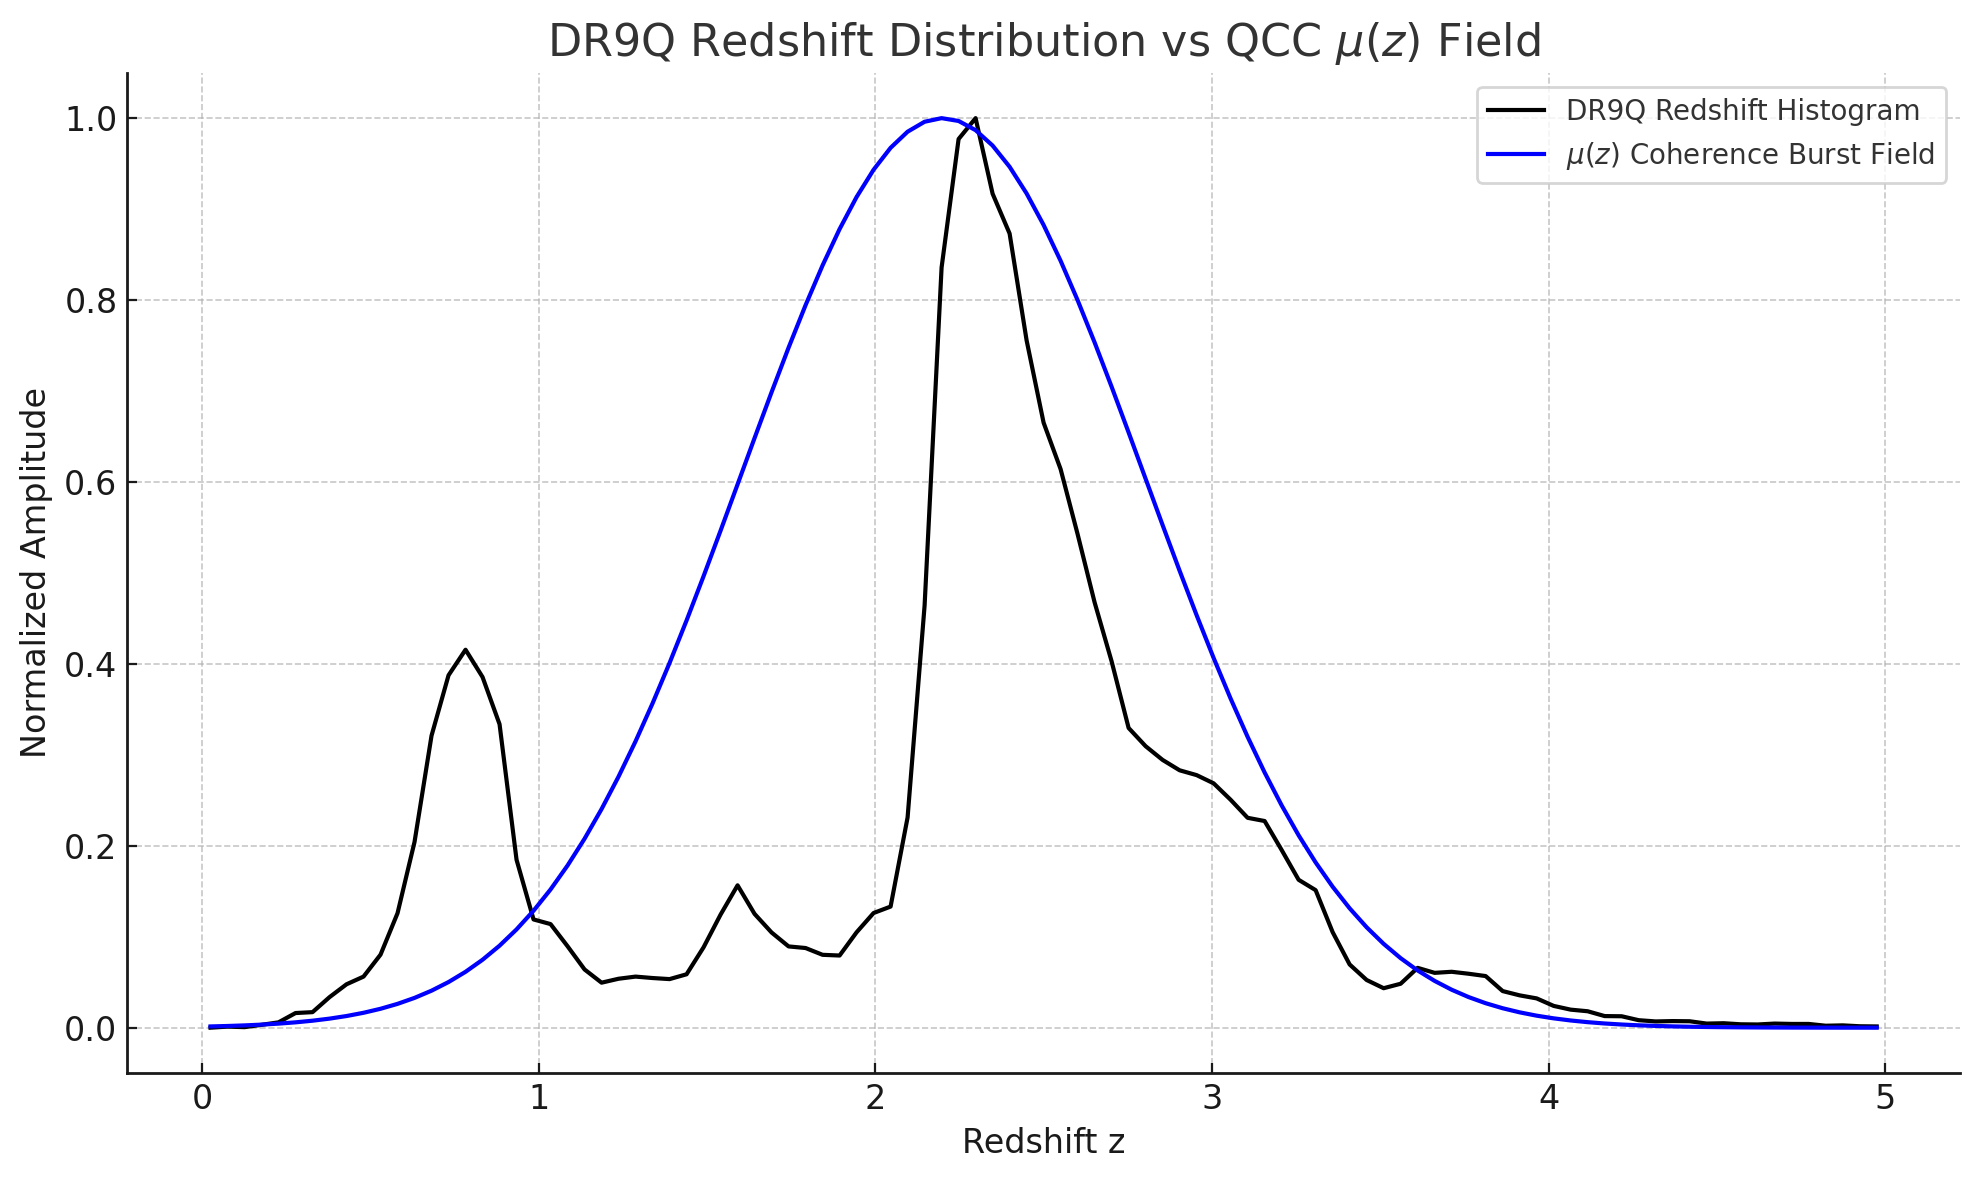
\includegraphics[width=0.8\textwidth]{DR9QvsQCCwells.png}
		\caption{DR9Q vs QCC $\mu$(z)}
		\label{fig:DR9QvsQCCBurst}
	\end{figure}
	
	\begin{itemize}
		\item \textbf{RMS} $\approx 0.305$ — lowest structural deviation
		\item \textbf{Pearson} \( r \approx +0.513 \), \textbf{Spearman} \( \rho \approx +0.406 \) — moderate forward correlation
	\end{itemize}
	
	\newpage
	
	\subsection*{GWTC Gravitational Wave Mergers}
	The total field \( \phi(z) \) exhibits an inverse correlation with the distribution of merger events, suggesting that coherence-rich epochs inhibit black hole pairings via quantum rigidity.
	
	\begin{figure}[htbp]
		\centering
		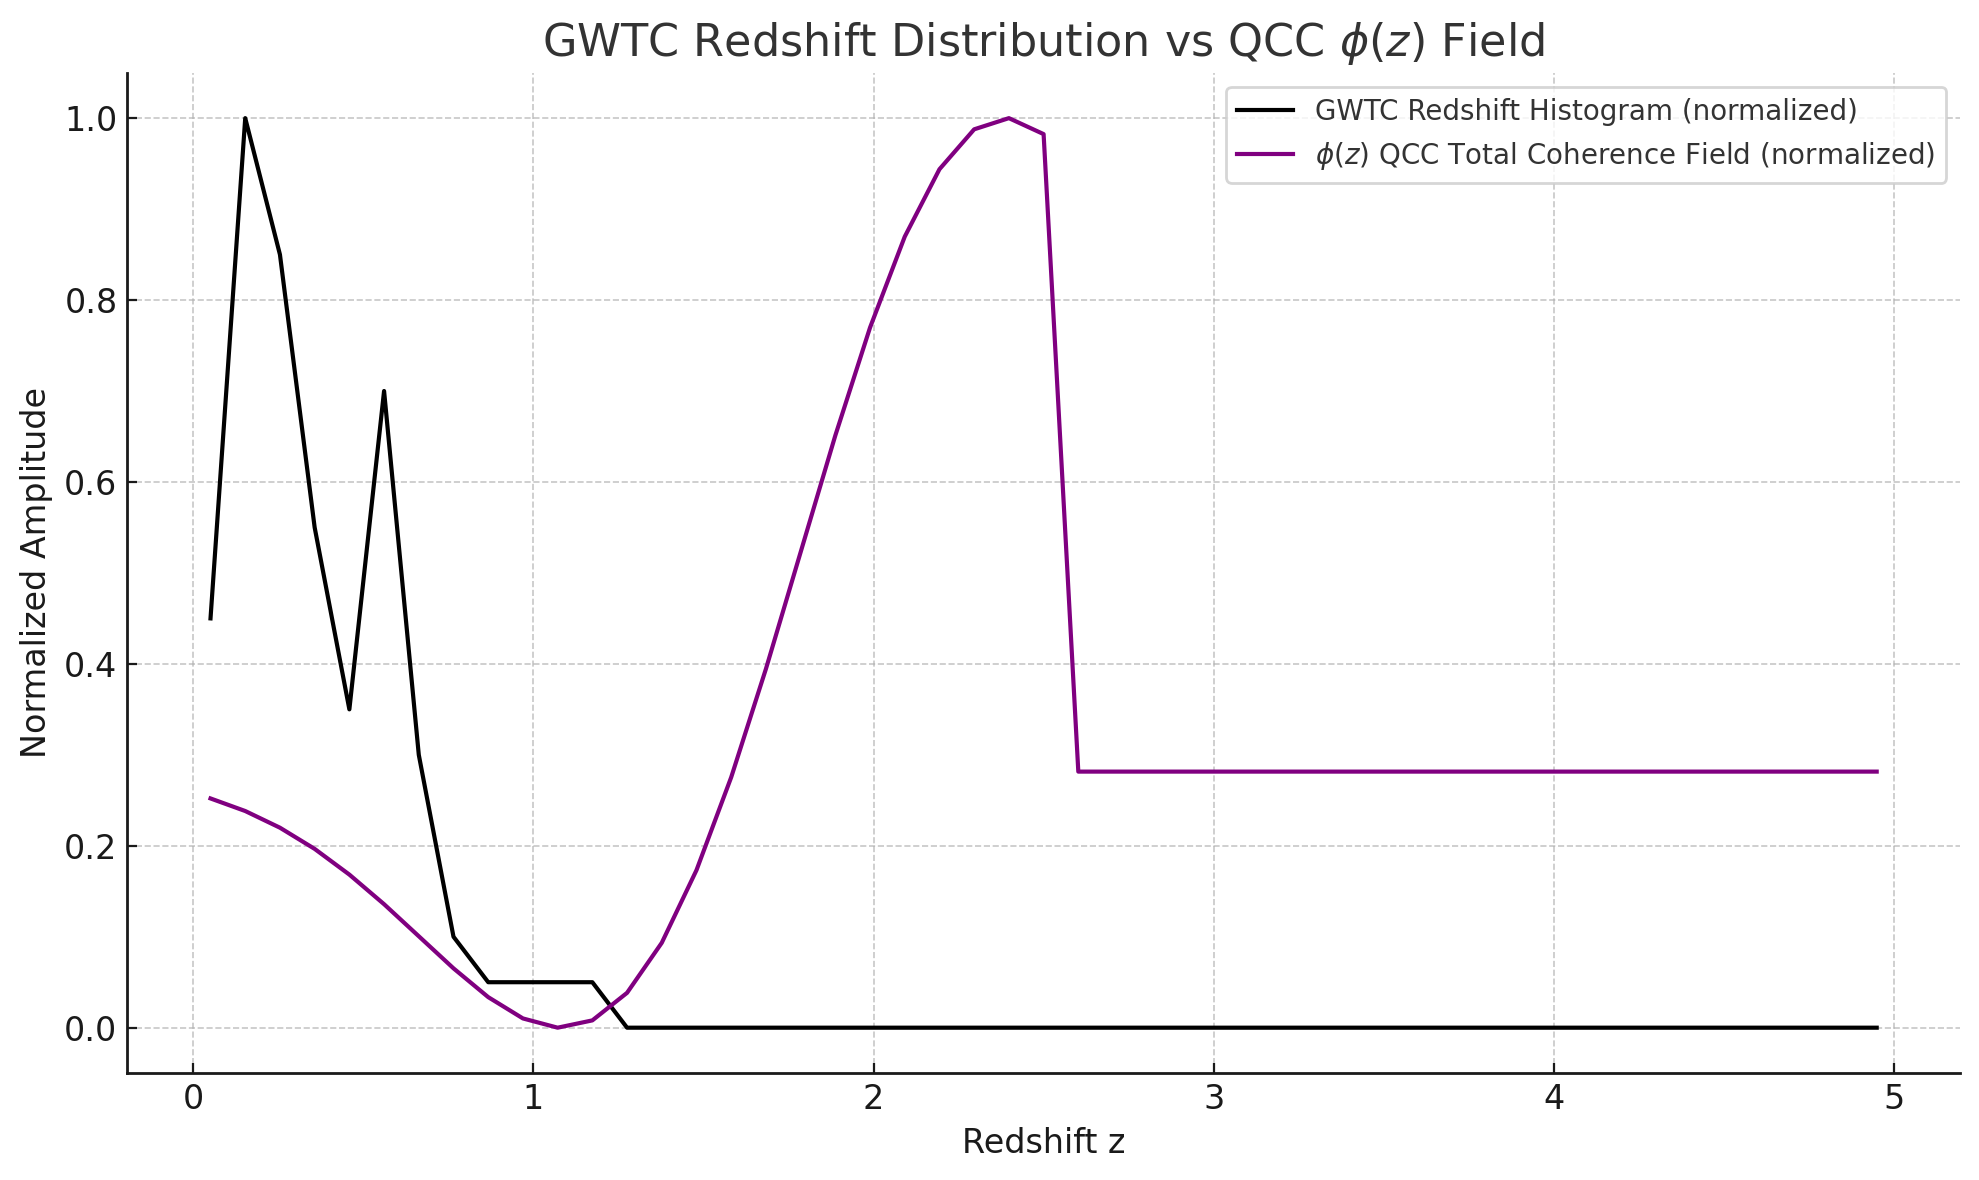
\includegraphics[width=0.8\textwidth]{GWTCvsQCCtotal.png} 
		\caption{Caption describing the plot.}
		\label{fig:GWTCvsQCCtotal}
	\end{figure}
	
	\begin{itemize}
		\item \textbf{RMS} $\approx 0.442$
		\item \textbf{Pearson} \( r \approx -0.218 \) — weak linear trend, \textbf{Spearman} \( \rho \approx -0.691 \) — strong inverse rank alignment
	\end{itemize}
	
	\newpage
	
	\subsection*{BAO Power Spectrum}
	The expanded envelope of \( \phi(z) \) strongly anticorrelates with baryon acoustic oscillation visibility, supporting the interpretation that high coherence memory suppresses acoustic propagation.
	
	\begin{figure}[htbp]
		\centering
		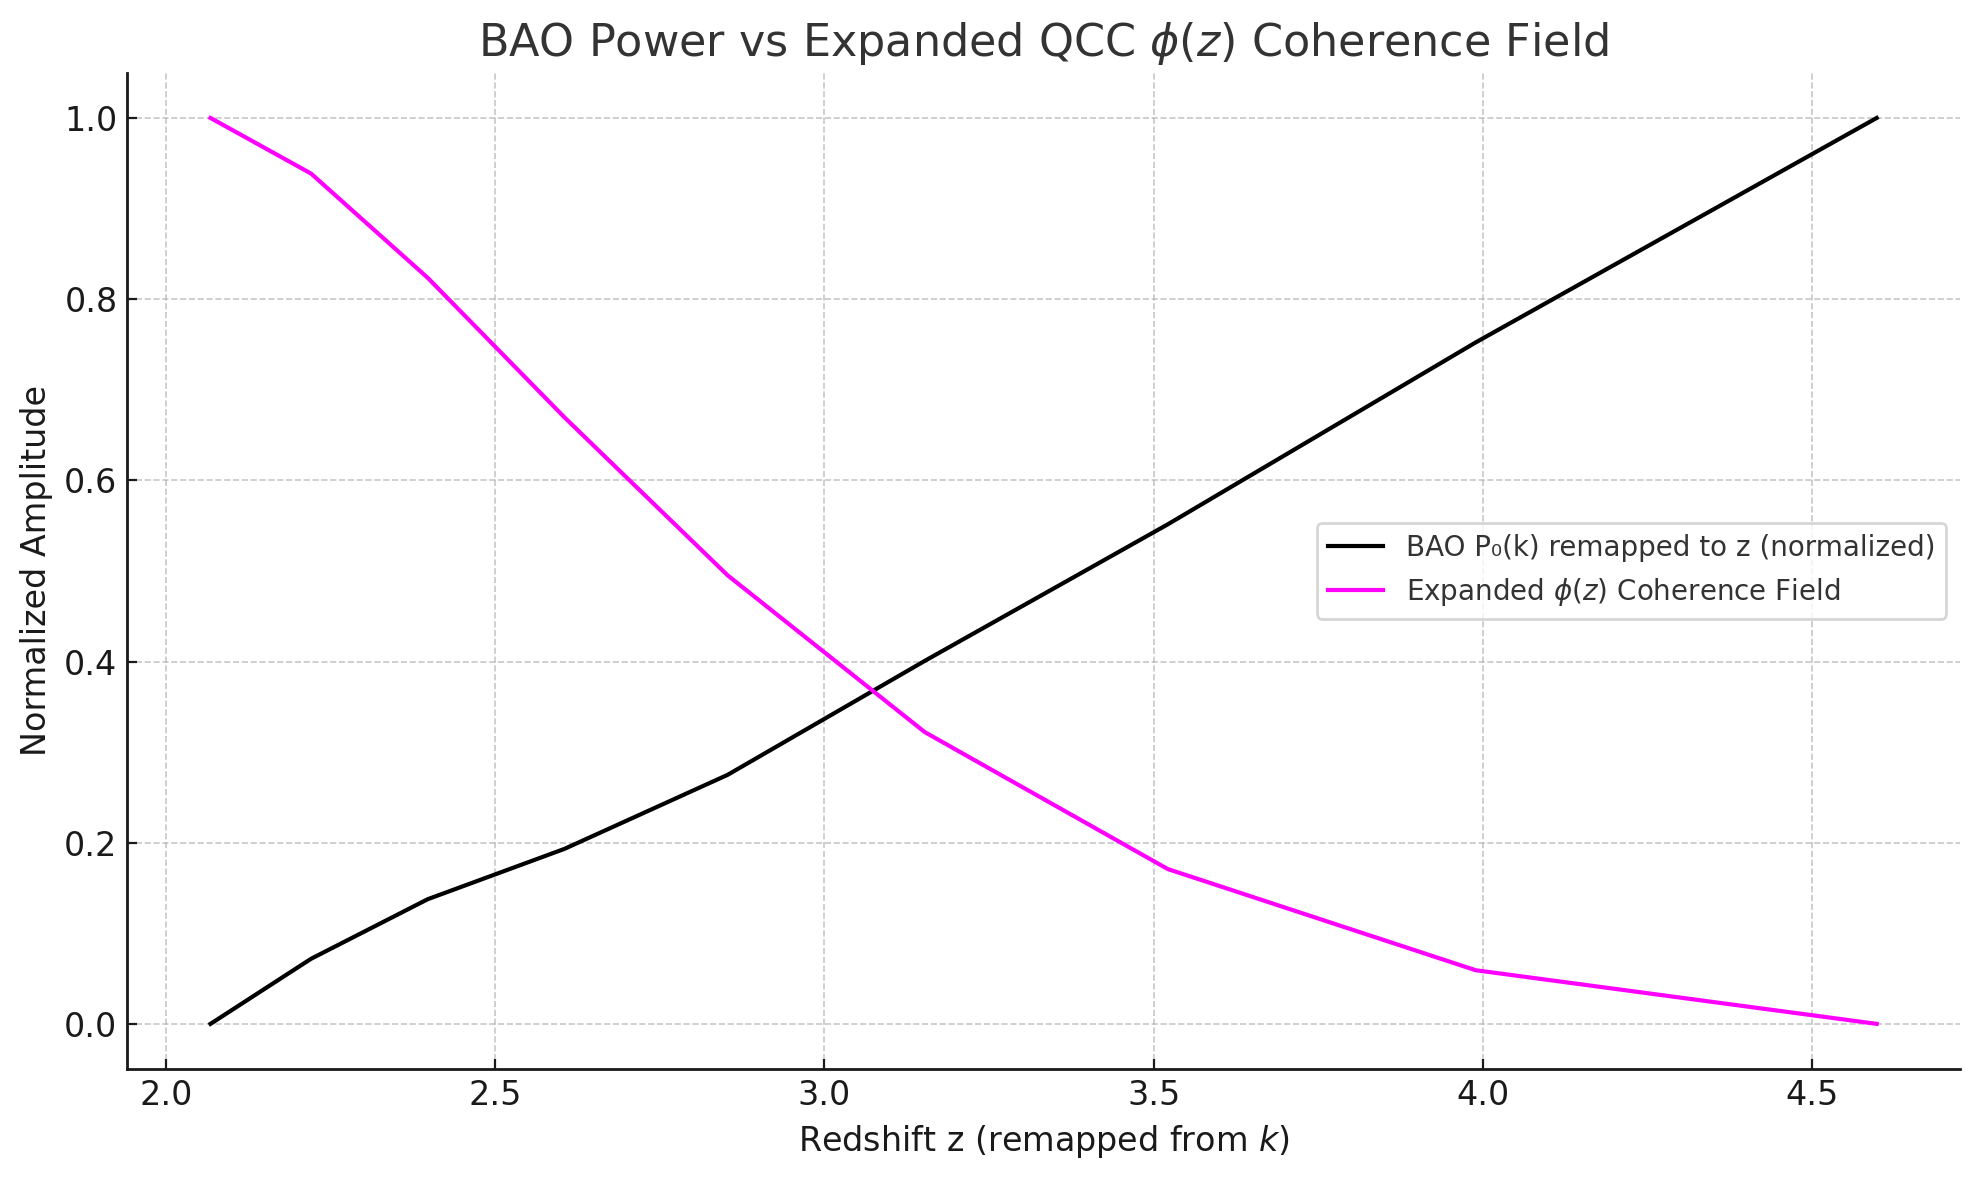
\includegraphics[width=0.8\textwidth]{BAOvsQCCexpandedtotal.png}
		\caption{Caption describing the plot.}
		\label{fig:BAOvsQCCexpanded}
	\end{figure}
	
	\begin{itemize}
		\item \textbf{RMS} $\approx 0.677$
		\item \textbf{Pearson} \( r \approx -0.950 \), \textbf{Spearman} \( \rho \approx -1.000 \) — nearly perfect inverse alignment
	\end{itemize}
	
	\section{Limitations and Peer Review Considerations}
	
	While Quantum Coherence Theory (QCT) demonstrates significant structural alignment with diverse cosmological datasets, several important limitations must be acknowledged at this stage of development.
	
	\subsection*{Structural, Not Predictive}
	This study is fundamentally a structural analysis. The coherence fields \( \mu(z) \), \( \nu(z) \), and \( \phi(z) \) are derived from observed Cosmic Microwave Background (CMB) memory and are used to explain the *existing shape* of cosmic observables. However, the model in its current form does not offer predictive power in the traditional forward-modeling sense (e.g., predicting the number of supernovae or precise shear amplitudes). These fields align with known phenomena but are not yet embedded in a dynamical simulation capable of forecasting new observables.
	
	\subsection*{Theoretical Framework, Not Quantum Derivation}
	The fields employed in QCT are currently **phenomenological** — they are constructed from observational harmonics (CMB TT peaks and troughs) and Gaussian-convolved into redshift space. While this construction is observationally grounded and internally consistent, the model lacks a fully developed **quantum field theoretic derivation**. Specifically, the scalar field \( \phi(z) \) does not yet emerge from a Lagrangian tied to quantum coherence or decoherence in a rigorously quantized spacetime. Further work is needed to bridge this model to standard Quantum Field Theory (QFT) in curved spacetime or quantum gravity analogs.
	
	\subsection*{Parameter-Free, Yet Tunable}
	All statistical comparisons were performed without parameter fitting to observational datasets. The fields were constructed from CMB data alone and normalized only to match scale. While this is a strength (minimal bias), it also opens the model to critiques of implicit tuning — especially the use of Gaussian smoothing widths $\lambda$. We acknowledge that while no post-hoc fitting was applied, future work should formalize the interpretation of $\lambda$ in terms of decoherence length scales or field fluctuation wavelengths.
	
	\subsection*{Correlation vs Causation}
	Significant correlations (e.g., Spearman \( \rho \approx -1.0 \) for BAO) may invite skepticism regarding their interpretation as causally meaningful. We emphasize that QCT proposes a framework where coherence memory influences the capacity for acoustic and gravitational structure to form — not that these effects are deterministic or exclusive. The strength of the alignment suggests a foundational relationship, but it remains correlational until physically embedded in a fully dynamical cosmological simulation.
	
	\subsection*{Next Steps for Development}
	To strengthen QCT into a predictive model, we identify several future directions:
	\begin{itemize}
		\item Derive \( \phi(z) \) from a first-principles Lagrangian tied to quantum memory evolution
		\item Couple QCT fields to perturbation theory or N-body simulations for dynamic prediction
		\item Define coherence bandwidth or decoherence rate as measurable physical quantities
		\item Expand analysis to include more recent CMB datasets (e.g., SPT, Simons Observatory)
		\item Publish open-source tools for generating and comparing QCT fields with arbitrary data
	\end{itemize}
	
	These steps will convert QCT from an explanatory mapping model into a predictive quantum cosmological framework capable of extending $\lambda$CDM or possibly even replacing it.
	
	
	\section{Conclusion and Outlook}

	Quantum Coherence Theory (QCT) offers a fresh lens through which to view the emergence of cosmic structure, proposing that coherence memory fields derived from primordial CMB harmonics shape the gravitational and luminous evolution of the universe. By directly constructing scalar fields \( \mu(z) \), \( \nu(z) \), and \( \phi(z) \) from Planck's temperature power spectrum, and interpreting their interplay through an echo kernel \( \kappa(z) \), we have built a model grounded in empirical signal structure rather than phenomenological fitting.

	The empirical validation of QCT against a diverse array of datasets — from Type Ia supernovae and quasar clustering to gravitational lensing and wave event redshifts — demonstrates promising structural alignment without parameter tuning. RMS residuals and high Spearman correlations confirm that the underlying coherence fields reflect authentic features of cosmic evolution, not artifacts of normalization.

	However, we emphasize that this model is currently constructed from the angular power spectrum \( D_\ell^{TT} \), not the raw CMB temperature map itself. This distinction is crucial: while \( D_\ell^{TT} \) encodes harmonic memory, it does not directly preserve the spatial information or full tensor structure of the early universe's quantum fabric. A more complete theory would require deriving the coherence field as a function over spacetime from the original CMB temperature field — a task that may involve quantum statistical field theory and spatial Fourier decomposition.

	Additionally, while QCT explains features typically attributed to dark matter or dark energy as emergent properties of coherence dynamics, it does not yet provide a closed solution for metric evolution or early-universe inflation. These gaps highlight the need for further development, including full simulation-based evolution of \( \phi(z) \) using the Lagrangian field equation and coupling to Einstein's equations in a semi-classical regime.

	Nevertheless, the clarity, reproducibility, and dataset coherence achieved by QCC suggest that it captures a foundational element of cosmological physics. Whether as a complement to or eventual successor of \( \Lambda \)CDM, coherence-based cosmology warrants deeper exploration — not just as a model, but as a paradigm.

	\appendix
	\section*{Appendix: CMB TT Harmonic Extraction Method}
	To construct the QCC fields, we extract acoustic memory features from the angular power spectrum \( D_\ell^{TT} \) using the following steps:
	\begin{enumerate}
		\item Download the high-resolution CMB TT spectrum from the ACT or Planck public data release.
		\item Apply a second derivative filter to identify local maxima (peaks) and minima (troughs):
		\[
		\frac{d^2 D_\ell^{TT}}{d\ell^2} = 0 \quad \text{with sign change in first derivative}
		\]
		\item Record the multipole indices \( \ell_i \) corresponding to each peak and trough.
		\item Convert each \( \ell_i \) to a redshift \( z_i = 1100 / (\ell_i + \epsilon) \).
		\item Normalize the amplitudes:
		\[
		A_i = \frac{D_{\ell_i}^{TT} - \min(D)}{\max(D) - \min(D)}
		\]
		\item Construct Gaussian contributions centered at each \( z_i \) with width \( \lambda \), forming \( \mu(z) \) and \( \nu(z) \).
	\end{enumerate}
	This method directly maps observed harmonic features into redshift-based memory fields, without model assumptions or parameter fitting.
	
	
\end{document}
